% options:
% thesis=B bachelor's thesis
% thesis=M master's thesis
% czech thesis in Czech language
% slovak thesis in Slovak language
% english thesis in English language
% hidelinks remove colour boxes around hyperlinks

\documentclass[thesis=B,czech]{FITthesis}[2012/06/26]

\usepackage[utf8]{inputenc} % LaTeX source encoded as UTF-8

\usepackage{graphicx} %graphics files inclusion
% \usepackage{amsmath} %advanced maths
% \usepackage{amssymb} %additional math symbols

\usepackage{dirtree} %directory tree visualisation

\usepackage{subfig}
\usepackage{listings}

%\hypersetup{unicode}

% % list of acronyms
% \usepackage[acronym,nonumberlist,toc,numberedsection=autolabel]{glossaries}
% \iflanguage{czech}{\renewcommand*{\acronymname}{Seznam pou{\v z}it{\' y}ch zkratek}}{}
% \makeglossaries

\newcommand{\tg}{\mathop{\mathrm{tg}}} %cesky tangens
\newcommand{\cotg}{\mathop{\mathrm{cotg}}} %cesky cotangens

% % % % % % % % % % % % % % % % % % % % % % % % % % % % % %
% ODTUD DAL VSE ZMENTE
% % % % % % % % % % % % % % % % % % % % % % % % % % % % % %

\department{Katedra \ldots softwarového inženýrství}
\title{Florbalový trenér}
\authorGN{Jakub} %(křestní) jméno (jména) autora
\authorFN{Olejník} %příjmení autora
\authorWithDegrees{Jakub Olejník} %jméno autora včetně současných akademických titulů
\supervisor{Ing. Josef Gattermayer}
\acknowledgements{Rád bych poděkoval Ing. Josefu Gattermayerovi za odborné vedení této práce a~trenérským kolektivům florbalových oddílů FbC Panthers a~AC Sparta Praha Florbal za spolupráci v~analytické části této práce.}
\abstractCS{Práce se zabývá vývojem mobilní aplikace pro tablety s~operačním systémem iOS, která si klade za cíl zjednodušit florbalovým trenérům přípravu florbalových tréninků a~cvičení. Uživatel, který aplikaci využívá, by se díky ní měl plně soustředit na obsah tréninkové jednotky nikoliv na formu, ve které ji zachytí, a~ve které ji bude následně prezentovat svým svěřencům.}
\abstractEN{The thesis deals with development of a mobile application for tablets with operating system iOS, which should simplify preparations of floorball trainings and exercises. User of this application should fully focus on the content of training unit, not the form in which it will be captured and then presented to his team.}
\placeForDeclarationOfAuthenticity{V~Praze}
\declarationOfAuthenticityOption{4} %volba Prohlášení (číslo 1-6)
\keywordsCS{florbal, trenér, trénink, iOS}
\keywordsEN{floorball, coach, training, iOS}

\begin{document}

% \newacronym{CVUT}{{\v C}VUT}{{\v C}esk{\' e} vysok{\' e} u{\v c}en{\' i} technick{\' e} v Praze}
% \newacronym{FIT}{FIT}{Fakulta informa{\v c}n{\' i}ch technologi{\' i}}

\begin{introduction}
	Informační technologie jsou dnes využívány téměř ve všech oblastech lidské činnosti, přesto se dají najít činnosti jimi nedotčené. Takovou oblastí jsou mladé a~zatím neolympijské sporty, které často doplácí na podmínky amatérského prostředí. Velmi často ani špičkové oddíly nejsou schopny nabídnout svým hráčům dostatečně kvalitní zázemí. Aplikace vyvíjená v~rámci této práce si klade za cíl tento nedostatek alespoň zmírnit.

	Toto téma jsem si zvolil na základě osobní zkušenosti a vědomí, že taková mobilní aplikace zatím neexistuje. Podobné názory jsem zaznamenal vždy, když jsem na toto téma diskutoval s~jinými florbalovými trenéry. Jejich reakce na vznik takové aplikace byly vždy kladné, a proto si myslím, že navržená aplikace bude využívána a mohla by pomoci zvednout kvalitu florbalových tréninků.
\end{introduction}

\chapter{Cíl práce}
	Výsledkem práce je funkční prototyp, kterým bude možné nahradit nyní využívané kreslicí tabule. Využitím tabletu se odstraní nutnost použití jiných kreslicích nástrojů, které nemusí být vždy dostupné, popř. jejich viditelnost na tabuli není dostačující. Dále elektronickou tabuli nelze umazat tak, aby na ní nebylo vysvětlované cvičení čitelné, v~případě umazání displeje jej lze snadno očistit.

	Naopak cílem práce není aplikace určená pro libovolné kreslení. Takovou aplikaci by samozřejmě bylo možné využít i pro výše zmíněné účely, nicméně podpora symboliky, která se mezi trenéry a hráči již nyní využívá, tvoří fundamentální základ celé aplikace a~je hlavním znakem, který tuto aplikaci odlišuje od ostatních, které ji mohou svým zaměřením připomínat.

	Vytvořená aplikace nemá podporovat veškerou funkcionalitu zmíněnou v~této práci, výsledná aplikace má poskytnout dobře fungující základ, který bude možné v~budoucnu rozšiřit i o~jiné než zde zmíněné funkce.

	Zároveň je důležité navrhnout odpovídající uživatelské rozhraní, které bude dostatečně jednoduché a intuitivní. Stejně tak rozhraní nesmí odporovat zvyklostem platformy iOS, aby se uživatel v~aplikaci neztratil již po prvním spuštění.

\chapter{Analýza}

	Na začátku práce byla provedena analýza problematiky. Byly zohledněny dobré i špatné vlastnosti již existujících aplikací nejen na iOS, ale i na OS Android a desktopových systémech. V~rámci analýzy bylo provedeno dotazníkové šetření na jehož základě, byl upraven seznam funkcí, které jsou, nebo budou implementovány. Na základě této analýzy vznikla specifikace požadavků, která bude v~této kapitole rozebrána.

\section{Analýza požadavků}

\subsection{Dotazníkové šetření}\label{sec:survey}

	V~rámci analytické části práce jsem se rozhodl oslovit vybraný vzorek potenciálních uživatelů aplikace. Primárním cílem tohoto šetření byla především kontrola, zda se podařilo zaměřit na opravdu důležité časti aplikace. Dalším z~cílů bylo získání povědomí o~podobných aplikacích, které již někdo za podobným účelem použil.

	Jednotlivé body dotazníku budou rozebrány v~této kapitole. Pro analýzu zmíněných podobných aplikací je připravena samostatná kapitola (\ref{sec:competition}).

\subsubsection{Cílové věkové kategorie} \label{sec:target_group}

	Jak je patrné z~grafu \ref{graph:category}, šetření prokázalo, že cílovou skupinou budou trenéři starších kategorií (starší žáci a výše) \-- u~mladších kategorií jsou priority nastaveny jinak, než u~těch starších. Mladší (popř. začínající) hráče je třeba naučit florbalové základy \-- postoj, držení hole, střela, přihrávka, což je nutné předvést, nikoli kreslit.

	\begin{figure}[h!t]
		\centering
		\includegraphics{img/graph_category}
		\caption{Graf trénovaných kategorií}\label{graph:category}
	\end{figure}

\subsubsection{Četnost užití kreslicí tabule}

	Dalším zjištěním (graf \ref{graph:table_usage}), které nebylo překvapením je fakt, že přibližně pouze pětina trenérů kreslicí tabuli nepoužívá vůbec, překvapením byla druhá část grafu \-- třetina trenérů ji využije více než pětkrát za trénink.

	Počet trenérů, kteří tabuli nevyužívají přibližně kopíruje počet trenérů, kteří trénují mladší kategorie, což potvrzuje tvrzení v~předchozí kapitole (\ref{sec:target_group}).

	\begin{figure}[h!t]
		\centering
		\includegraphics{img/graph_table_usage}
		\caption{Graf využítí kreslicí tabule}\label{graph:table_usage}
	\end{figure}

\subsubsection{Funkce volné kreslení, seskupování cvičení, perzistence}

	Výsledky potvrdily, že funkce volného kreslení (jako v~Malování v~MS Windows) je pro uživatele nepostradatelná. Toto od začátku měla být základní funkcionalita aplikace. Stejně zásadními se ukázaly funkce perzistentního uložení a funkce seskupování cvičení do tréninků. Seskupování bylo od začátku považováno za důležitou funkcionalitu, ale podle tohoto výsledku bylo rozhodnuto o~jeho zařazení do aplikace.

\subsubsection{Textové poznámky}

	Naopak překvapením bylo, že textové poznámky nejsou pro trenéry tak důležité, třetina dotázaných by se bez nich obešla. Nicméně tato funkcionalita byla do aplikace zařazena, protože poznámkový aparát může sloužit jako upomínka pro trenéra, aby nezapomněl, co je důležité hráčům před cvičením zdůraznit, což vede k~jejich růstu.

	Dalším důležitým faktorem je, že poznámky mohou do jisté míry nahradit funkcionalitu, která vyplynula z~dotazníkového šetření jako chtěná (např. docházka), ale prozatím byla odložena. Tímto způsobem je možné ji nahradit bez časového zdržení a  implementačních komplikací.

\subsubsection{Automatické nakreslení cvičení}

	Zajímavou funkcionalitou, kterou by bylo dobré jednou v~aplikaci mít, je automatické postupné nakreslení cvičení. Tato funkce snižuje nároky na prezentační schopnosti trenéra tím, že jednoduchým poklepáním je schopen připravené cvičení \uv{nakreslit}. Zároveň jsou sníženy nároky na grafické schopnosti na trenéra, protože nemusí ve spěchu a v~nepohodlné pozici cvičení kreslit. Tato funkce se líbila všem dotázaným a je na seznamu funkcí, které budou do aplikace v~nejbližší době doplněny. Takto bylo rozhodnuto z~důvodu její pracnosti a omezené časové dotaci na tuto práci.

	Toto byl výčet původně navrhovaných funkcí, které by měly být v~aplikaci implementovány, následující funkce jsou tipy, které by dotazovaní trenéři v~aplikaci ocenili.

\subsubsection{Elektronická tužka}

	Jednou z~navrhovaných funkcionalit je možnost vkládání videí a jejich následný rozbor, tzv. \uv{elektronická tužka}. Tato funkce bude z~aplikace kompletně vynechána. Taková funkcionalita nepatří do aplikace tohoto typu, protože aplikace se zabývá přípravou cvičení a jeho případnému vysvětlení a elektronická tužka je poněkud jiného typu.

\subsubsection{Docházka}

	Další zmíněnou funkcí byla docházka na trénink. Tato funkce nebude implementována, protože nesouvisí s~přípravou tréninku. Tato funkce by mohla být zařazena do kategorie \uv{managementu} tréninku, což odporuje zamýšlenému určení aplikace.

	Dalším aspektem pro vynechání funkce byl fakt, že trenér má možnost si docházku zapsat. K~tomuto účelu může využít textové poznámky, které budou v~aplikaci implementovány, a jsou mu tedy dostupné.

\subsubsection{Čas, který cvičení zabralo}

	Toto může být užitečná informace, např. ke zpětnému zhodnocení, zda bylo dobré cvičení zařadit do tréninku. Návrh vhodné implementační varianty by nejspíše vedl k~rozlišení různých typů poznámek, což by mohlo být užitečné. V~aktuální verzi aplikace různé typy poznámek nebudou zavedeny. To ale neznamená, že uživatel nutně o~tuto informaci přijde, stále bude mít možnost si tento čas zapsat do textové poznámky.

\subsubsection{Sdílení cvičení a tréninků}

	Tato funkce již dříve byla na seznamu funkcí k~prioritní implementaci. V~první verzi aplikace toto podporováno nebude. Důvodem k~tomuto rozhodnutí byl fakt, že k~funkčnímu a pohodlnému sdílení by bylo nutné zařídit server, který by měl na starosti databázi sdílených cvičení.

	Také by se mohlo snadno stát, že místo základních funkcí, za které jsou považovány volné kreslení a užívání připravených nástrojů, by se přednostně implementovala síťová komunikace, což by mohlo vyústit v~nedodržení termínu práce.

\subsubsection{Duplikace cvičení}

	Užitečnou funkcí, která se mezi odpověďmi objevila byla snadná duplikace cvičení. Motivací k~takové funkcionalitě je zkušenost, že velké množství cvičení, se liší pouze v~malých detailech, např. přihrávka navíc, pohyb navíc. A~tak je nepraktické kreslit celé cvičení znovu, pokud je možnost cvičení zduplikovat a přihrávku přikreslit.

\subsection{Podporovaná zařízení}

	Operační systém iOS patří mezi velmi dynamicky se rozvíjející platformy, několikrát do roka je vydána nová verze, která obsahuje nové funkce. Toto samozřejmě může přinášet problémy se zpětnou kompatibilitou, nicméně velká většina zařízení vždy přejde na novou verzi systému téměř okamžitě, tudíž roztříštěnost tohoto systému prakticky neexistuje, což samozřejmě přináší vývojářům spoustu výhod.

	Poslední verze (verze 7) přinesla velké množství změn, především v~uživatelském rozhraní, proto bylo rozhodnuto podporu starších verzí systému z~aplikace vynechat. Důležité přitom je, že poslední verzi systému používá vetšina uživatelů, což znázorňuje graf \ref{graph:ios7_stats} \cite{devAppleStats}.

	\begin{figure}[h!t]
		\centering
		\includegraphics{img/ios7stats}
		\caption{Graf verzí iOS k~27.4.2014 \cite{devAppleStats}}\label{graph:ios7_stats}
	\end{figure}

	Podpora pouze pro zařízení s~iOS 7 znamená, že podporovanými zařízeními jsou iPhone 4 a novější, iPad 2 a novější. Protože aplikace cíli pouze na tablety, nikoliv na mobilní telefony, jsou podporována pouze zařízení iPad 2 a novější \cite{ios7compat}.

\section{Podobné aplikace}\label{sec:competition}

	V~rámci analýzy požadavků bylo nutné prozkoumat, zda existují podobné aplikace. Následně v~nalezených aplikacích bylo potřeba identifikovat jejich kladné, ale i záporné vlastnosti. Takto získané informace byly následně využity pro zlepšení navrhnované aplikace.

	Analýza podobných aplikací byla zaměřena především na uživatelské rozhraní nalezených aplikací a funkce, které aplikace nabízí. U~funkcí bylo důležitým kritériem, zda jsou užitečné pro florbalové trenéry.

	\subsection{CoachNote Hockey And Ringette \cite{coachnoteAppstore}}

	Tato aplikace\footnote{v době analýzy byla dostupná verze 1.6.6} se od začátku analýzy jevila jako nejkvalitnější ze všech nalezených. Zároveň se svým zaměřením i nabízenou funkcionalitou zaměřovala na podobnou cílovou skupinu uživatelů jako aplikace navrhovaná v~této práci.

	\begin{figure}[h!t]
		\centering
		\includegraphics[width=\textwidth]{img/competition/coachnote/IMG_0015}
		\caption{Hlavní menu aplikace CoachNote Hockey And Ringette}
		\label{pic:coachnote_menu}
	\end{figure}

	Uživatelské rozhraní (obr. \ref{pic:coachnote_menu} a \ref{pic:coachnote_exercises}) vypadá podle mého názoru líbivě, nicméně toto je vykoupeno jeho nižší intuitivitou. Aplikace nabízí velké množství funkcí, které je občas složité dohledat. Zároveň ikony, které byly zvoleny pro nástroje mohou uživatele zmást (např. ikona pro skrytí panelu nahrávaní zvuku).

	Rozšířené možnosti jednotlivých nástrojů jsou dostupné po druhém tapnutí na zvolený nástroj. Toto řešení považuji za nešťastné, jelikož jiné kreslicí nástroje, nejen na platformě iOS, řeší tyto věci jiným způsobem, např. změnou položek ve speciálním panelu, který je pro rozšířená nastavení zvoleného nástroje určen. Z~tohoto důvodu si myslím, že uživatel často rozšířené možnosti nástroje nenajde.

	\begin{figure}[h!t]
		\centering
		\includegraphics[width=\textwidth]{img/competition/coachnote/IMG_0011}
		\caption{Zobrazení cvičení v~aplikaci CoachNote Hockey And Ringette}
		\label{pic:coachnote_exercises}
	\end{figure}

	Po stránce dostupných funkcí by aplikace florbalovému trenérovi mohla vyhovovat. Nicméně pro zobrazení hráčů využívá jinou notaci \-- odlišuje je pouze pomocí barev, což je mezi florbalovými trenéry podle mého názoru nedostačující, protože trenéři i hráči jsou zvyklí rozlišení pomocí různých symbolů.

	U~aplikace je šikovné, že hráči jsou speciální objekty, které je možné přesouvat a aplikace zobrazuje jejich trajektorii. Bohužel tato funkce není dotažena do konce a hráče lze přesunout pouze z~bodu A~do bodu B, pokud je potřeba jej přesunout do dalšího bodu, pak jeho předchozí trajektorie zmizí.

	Aplikace obsahuje velké množství funkcí, některé jsou podle mého názoru zbytečné (např. nahrávání zvuku) a jiné důležité chybí. Jednou z~takových funkcí, kterou se mi nepodařilo dohledat je mazání jednotlivých hráčů. Aplikace nabízí pouze možnost smazat všechny hráče, kteří jsou na hřišti zakresleni, což považuji za velký nedostatek, obzvlášť pokud uvažujeme, jak je aplikace komplexní.

	Analýza této aplikace byla zaměřena především na verzi, která je dostupná zdarma na \href{https://itunes.apple.com/us/app/coachnote-hockey-ringette/id562205341?mt=8}{App store}. Placená verze aplikace je osvobozena od reklamy a obsahuje rozšířenou funkcionalitu (např. možnost psát text přímo do cvičení).

	Aplikace podporuje i zařízení iPhone, nicméně na tomto zařízení aplikace zkoušena nebyla, poněvadž navrhovaná aplikace se zaměřuje pouze na iPad.

	Existují různé varianty aplikace, které jsou zaměřené na jiné sporty. Ostatní varianty nebyly testovány, protože sporty, na které byly zaměřeny se od florbalu významně liší.

	Aplikace je poměrně kvalitní, při doplnění florbalové notace a po úpravě uživatelského rozhraní by mohla být dobře použitelná. Co by mohlo být pro uživatele nepříjemné, je až příliš dlouhé čekání při otevření prázdného cvičení\footnote{vyzkoušeno na iPadu 4 a na iPadu Air}.

	\subsection{IceHockey Board Free \cite{iceHockeyBoardAppstore}}

	Aplikace \footnote{v~době analýzy byla dostupná verze 8.4} je zdarma dostupná na \href{https://itunes.apple.com/ca/app/icehockey-board-free/id366079177?mt=8}{App store}. Aplikace je zaměřena na lední hokej, existují varianty pro jiné sporty, např. pozemní hokej, ale varianta pro florbal chybí.

	Aplikace je velmi jednoduchá, obsahuje pevný počet hráčů (6 pro každý z~týmů). Aplikace si umí ukládat pozice hráčů a poté mezi těmito uloženými stavy lze tapnutím přecházet. Toto platí pouze pro pozice hráčů, nakreslené čáry jsou zobrazeny vždy, bez ohledu na uložený stav.

	Uživatelské rozhraní (obr. \ref{pic:icehockey_board_free}) v~aplikaci je minimalistické, po spuštění se zobrazí hřiště a lze s~ním ihned manipulovat. Jednotlivé nástroje jsou dostupné po rozvinutí pomocného panelu, který je naznačen vhodnou ikonou.

	\begin{figure}[p]
		\centering
		\includegraphics[width=\textwidth]{img/competition/icehockey_board_free/IMG_0018}
		\caption{Uživatelské rozhraní aplikace IceHockey Board Free}
		\label{pic:icehockey_board_free}
	\end{figure}

	Po funkční stránce je aplikace příliš jednoduchá, neumožňuje mazání jednotlivých čar, mazat lze pouze všechny čáry hromadně. Na aplikaci je hezké, že umožňuje automatické nakreslení cvičení, avšak tato funkcionalita není dotažena a týká se pouze pozic jednotlivých hráčů. Tato aplikace posloužila pouze jako příklad, jak by navrhovaná aplikace neměla vypadat, rozhraní není pro uživatele přívětivé a funkce jsou omezené a nedotažené. Dále aplikace obsahuje pro uživatele velmi nepříjemnou reklamu, která jej zdržuje od užívání při spuštění a při každé maximalizaci aplikace.

	\newpage

	\subsection{My Field Hockey Coach Free \cite{myFieldHockeyAppstore}}

	Verze aplikace\footnote{v době analýzy byla dostupná verze 3.1}, která je dostupná zdarma na \href{https://itunes.apple.com/us/app/my-field-hockey-coach-free/id457826679?mt=8}{App store} je velice omezená, je zaměřená na pozemní hokej. Umožňuje pouze správu jednotlivých hráčů v~týmu a jejich rozmístění do formace. Další funkce této aplikace neodpovídají zaměření navrhované aplikace \-- jedná se o~možnost zobrazení ukazatele aktuálního skóre utkání a tabule složící k~signalizaci střídání. Aplikace neumožňuje žádnou formu kreslení. Toto by mohlo být obsahem placené verze.

	\begin{figure}[h!t]
		\centering
		\subfloat[Hlavní nabídka]{\includegraphics[width=0.4\textwidth]{img/competition/my_field_hockey_coach_free/IMG_0019}}
 		\hfil
 		\subfloat[Správa hráčů]{\includegraphics[width=0.4\textwidth]{img/competition/my_field_hockey_coach_free/IMG_0021}}

 		\caption{Uživatelské rozhraní aplikace My Field Hockey Coach Free}
 		\label{pic:my_field_hockey_coach_free}
	\end{figure}

	Aplikace má povedené uživatelské rozhraní (obr. \ref{pic:my_field_hockey_coach_free}). Často jsou pro tlačítka použity textové popisky, čímž je možné se vyvarovat použití matoucích ikon.

	Bylo by dobré se inspirovat návrhem jednotlivých nabídek v~menu, které jsou navrženy přehledně a intuitivně. Naopak rozhraní pro kreslicí plochu v~aplikaci chybí, tudíž jej nelze jakkoliv analyzovat.

	\subsection{Exercise drawer \cite{exerciseDrawerOnline}}

	Aplikace psaná v~Javě, tudíž běžící na desktopových platformách, volně dostupná na \href{http://floorballcoach.org/exercisedrawer/}{internetu}. Jedná se o~aplikaci, která byla zmíněna v~dotazníkovém šetření (kapitola \ref{sec:survey}). Aplikaci považuji vhodnou na přípravu materiálů, pokud autor chce např. publikovat knížku o~trénování.

	Funkcemi se aplikace velmi podobá aplikaci navrhované v~této práci. Jako jediná je zaměřena na florbal. Nicméně některé funkce jsou omezené, např. je možné kreslit pouze úsečky \-- funkce volného kreslení chybí. Aplikace neumožňuje přípravu celých tréninků, je možné ukládat cvičení pouze jednotlivě. Je možné ke cvičení vkládat poznámky a to dvojím způsobem. Prvním je možnost vkládat poznámky přímo na plochu cvičení, druhá je možnost připsat právě jednu poznámku a uložit ji jako přílohu ke cvičení.

	Aplikace dále umí zobrazit mnoho typů hřiště, nicméně všechny typy jsou pouze mírně obměněné varianty nákresu celého hřiště a poloviny hřiště.

	Po funkční stránce mě zklamalo, že v~aplikaci nelze, popř. není snadné, smazat nakreslenou přihrávku, střelu ani pohyb hráče. Bylo možné smazat pouze hráče či kužel.

	\begin{figure}[h!t]
		\centering
		\includegraphics[width=\textwidth]{img/competition/exercise_drawer}
		\caption{Uživatelské rozhraní aplikace Exercise Drawer}
		\label{pic:exercise_drawer}
	\end{figure}

	Uživatelské rozhraní aplikace (obr. \ref{pic:exercise_drawer}) je jednoduché a přehledné, což připisuji především zvolené platformě a velikosti monitoru, na kterém byla aplikace zkoušena.

	Tato aplikace je co se týče funkční stránky pravděpodobně nejlepší a bylo by dobré, aby navrhovaná aplikace byla jejím ekvivalentem na platformě iOS.

	\subsection{Aplikace zmíněné v~dotaznících}

	V~provedeném dotazníkovém šetření \ref{sec:survey} byly zmíněny ještě další aplikace \-- Florbalový trenér a CoachAp (obě pro OS Android), nicméně ani jednu nebylo možné na Google Play Store nalézt, tudíž nebyly analyzovány.

	\section{Případy užití}

	Výsledkem analýzy je seznam případů užití (obr. \ref{pic:use_case}) , které budou v~navrhované aplikaci implementovány.

	\begin{itemize}
		\item zobrazení cvičení
		\item vytvoření cvičení
		\item duplikace cvičení
		\item úprava cvičení
		\item odstranění cvičení

		\item vložení elementu z~toolboxu
		\item kreslení na hřiště
		\item smazání prvku ze hřiště
		\item přidání poznámky
		\item úprava poznámky
		\item odstranění poznámky

		\item vytvoření tréninku
		\item přidání cvičení do tréninku
		\item odstranění cvičení z~tréninku
		\item odstranění tréninku
	\end{itemize}

	\begin{figure}[h!t]
		\centering
		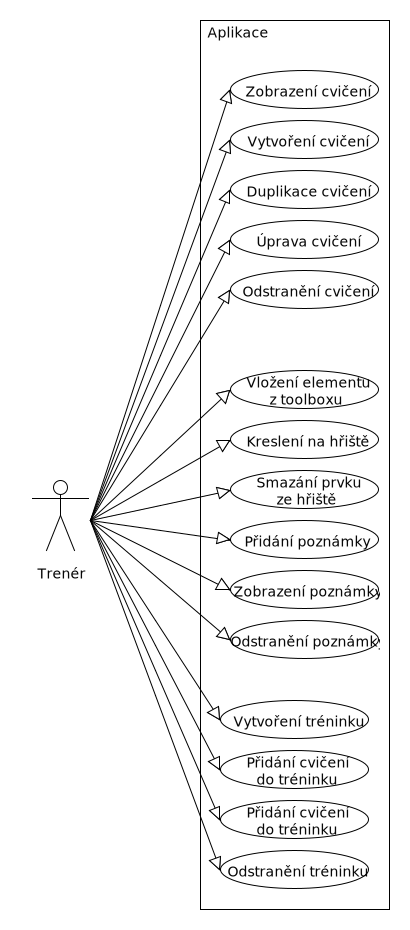
\includegraphics[width=\textwidth]{img/use_case}
		\caption{Diagram případů užití}
		\label{pic:use_case}
	\end{figure}

\chapter{Návrh}

	Tato kapitola se zaměřuje na obecnou strukturu iOS aplikací a jejich doporučenou architekturu. Dále zde bude rozebrán návrh uživatelského rozhraní, které často rozhoduje o~použitelnosti celé aplikace. Dalším bodem této kapitoly je návrh architektury.

	\section{Základy aplikací pro iOS}

	Aplikace pro platformu iOS jsou psané v~jazyce Objective-C, což je nadstavba standardního jazyka C, doplněná o~možnosti objektově orientovaného programování. Objective-C tedy doplňuje syntaxi jazyka C o~možnosti rozšíření pomocí tříd a metod. V~iOS aplikacích tedy lze využívat nejen vlastností jazyka Objective-C, ale i jazyka C. V~Objective-C je zároveň implementován koncept zasílání zpráv podobný tomu, který využívá jazyk Smalltalk. \cite{aboutObjCOnline}

	Aplikace se dá rozdělit na tři části: zdrojové kódy, resources a metadata aplikace.

	Ve zdrojových kódech se definuje vlastní chování aplikace. Jedná se o~hlavičkové soubory\footnote{typicky se jedná o~soubory s~příponou .h}, ve kterých je deklarováno veřejné rozhraní objektů, popř. jsou zde deklarovány veřejně dostupné funkce. Rozhraní metod (a funkcí) zahrnuje její název, návratovou hodnotu a její argumenty.

	Mezi zdrojové kódy se dále zahrnují implementační soubory\footnote{v jazyce C mají typicky příponu .c, v~Objective-C mají příponu .m}. Tyto soubory již definují chování veřejných metod a lze v~nich definovat metody, které by měly být privátní, nicméně takto definované privátní metody lze zavolat z~objektů jiných tříd, což je umožněno konceptem zasílání zpráv, který je v~tomto jazyce využíván.

	Do resources lze zahrnout soubory, které nemohou, nebo by neměly být součástí zdrojových kódů. Typicky se jedná o~soubory, které by měly být lokalizovány, což mohou být např. textové řetězce, které se v~aplikaci objevují, dále to mohou být obrázky, videa a podobné soubory. Takové soubory jsou vloženy do archivu aplikace, která je poté může využívat. Správné využití resources zvyšuje pružnost aplikace. Pokud je potřeba do aplikace přidat podporu pro nový jazyk, vyměnit využívané ikony, lze toho poté docílit bez jediného zásahu do kódu aplikace.

	Metadata aplikace jsou uložena v~XML souboru a obsahují informace např. o~názvu aplikace, o~jejím systémovém identifikátoru apod. Tato data jsou poté využita např. v~hlavní nabídce zařízení. \cite{plistKeysOnline}

	Aplikace pro iOS jsou založeny na architektuře Model-View-Controller (MVC). Tato architektura se vyznačuje tím, že každy objekt v~aplikace vystupuje v~jedné z~rolí (model, view, controller). \cite{appleMVCOnline}

	\begin{figure}[h!t]
		\centering
		\includegraphics[width=\textwidth]{img/model_view_controller}
		\caption{MVC: komunikace objektů \cite{appleMVCOnline}}
		\label{pic:mvc_communication}
	\end{figure}

	\subsection{Model}

	Modelové objekty zajišťují přístup k~datům aplikace a případnou manipulaci s~nimi. V~navrhované aplikaci se bude jednat např. o~objekt, který bude udržovat seznam uložených cvičení. Modelové objekty mohou obsahovat další modelové objekty, se kterými mohou komunikovat. V~navrhované aplikaci modelová třída, která bude udržovat seznam cvičení, bude obsahovat cvičení samotná, což je opět modelová třída.

	Správně navržený modelový objekt by měl pracovat pouze s~daty, neměl by být nijak propojen s~view, nebo s~controllerem. Takovýto správný návrh umožňuje jeho opětovné využití při řešení podobného problému.\cite{appleMVCOnline}

	\subsection{View}

	View objekty jsou objekty, která jsou pro uživatele viditelné. Tyto objekty zároveň umí zpracovat akce uživatele a přes controller je promítají do modelu. Stejně tak zkrze controller se view doví o~změnách dat v~modelu a může podle nich zareagovat.

	\subsection{Controller}

	Jedná se o~objekty, které zajišťují komunikaci mezi view a modelem, např. od view se controller doví o~změně, zajistí, aby se model o~takové změně dověděl a zareagoval na ni, pokud je to dále vyžadováno, tak změna v~modelu spustí akci controlleru, který zajistí, aby na ni zareagovalo opět i view.

	Controller zároveň může plnit i inicializační funkce, protože může spravovat životní cyklus jiných objektů, např. view.

	\section{Návrh uživatelského rozhraní}

	Uživatelské rozhraní, které bude aplikace využívat by mělo být velmi jednoduché, aby uživatel nepřemýšlel, kde najde vyžadovanou funkcionalitu. Zároveň by rozhraní mělo odpovídat zvyklostem platformy iOS, aby se uživatel v~aplikaci ihned po prvním otevření neztratil. Z~tohoto důvodu budou v~aplikaci použity standardní systémové komponenty, které budou doplněny vhodnými ikonami a barevným stylem.

	Pro vizualizaci rozvržení jednotlivých prvků v~aplikaci byly vytvořeny wireframy (obr. \ref{pic:wireframes1.1}, \ref{pic:wireframes1.2}, \ref{pic:wireframes1.3}, \ref{pic:wireframes1.4}) \cite{moqupsOnline}. Nicméně prvotní wireframy nereflektovaly požadavky uživatele, tudíž bylo potřeba je upravit (obr. \ref{pic:wireframes2}). Pozměněna byla obrazovka náhledu cvičení, která byla zjednodušena a zpřehledněna.

	\begin{figure}[h!t]
		\centering
		\subfloat[Hlavní nabídka]{\includegraphics[width=0.4\textwidth]{img/wireframes/1/menu}}
 		\hfil
 		\subfloat[Seznam cvičení]{\includegraphics[width=0.4\textwidth]{img/wireframes/1/seznam_cviceni}}
 		\caption{Návrh obrazovek aplikace, část 1}
 		\label{pic:wireframes1.1}
 	\end{figure}
 	\begin{figure}[h!t]
 		\centering
 		\subfloat[Seznam tréninků]{\includegraphics[width=0.4\textwidth]{img/wireframes/1/seznam_treninku}}
 		\hfil
 		\subfloat[Vytvoření tréninku]{\includegraphics[width=0.4\textwidth]{img/wireframes/1/pripravit_novy_trenink}}
 		\caption{Návrh obrazovek aplikace, část 2}
		\label{pic:wireframes1.2}
 	\end{figure}
 	\begin{figure}[h!t]
 		\centering
 		\subfloat[Náhled cvičení]{\includegraphics[width=0.4\textwidth]{img/wireframes/1/nahled_cviceni}}
 		\hfil
 		\subfloat[Seznam poznámek]{\includegraphics[width=0.4\textwidth]{img/wireframes/1/nahled_cviceni_seznam_poznamek}}
 		\caption{Návrh obrazovek aplikace, část 3}
 		\label{pic:wireframes1.3}
 	\end{figure}

 	\begin{figure}[h!t]
 		\centering
 		\subfloat[Detail poznámky]{\includegraphics[width=0.4\textwidth]{img/wireframes/1/nahled_cviceni_detail_poznamky}}
 		\hfil
 		\subfloat[O aplikaci]{\includegraphics[width=0.4\textwidth]{img/wireframes/1/o_aplikaci}}
 		\caption{Návrh obrazovek aplikace, část 4}
 		\label{pic:wireframes1.4}
	\end{figure}

	\begin{figure}[h!t]
		\centering
 		\subfloat[Náhled cvičení]{\includegraphics[width=0.4\textwidth]{img/wireframes/2/nahled_cviceni_2}}
 		\hfil
 		\subfloat[Seznam poznámek]{\includegraphics[width=0.4\textwidth]{img/wireframes/2/nahled_cviceni_poznamky}}

 		\caption{Upravený návrh uživatelského rozhraní}
 		\label{pic:wireframes2}
	\end{figure}

\section{Návrh architektury}

	Vhodná volba architektury ovlivňuje schopnost aplikace reagovat na pozdější změny. Při špatné volbě se mohou budoucí změny stát časově i finančně velice náročné. Při výběru architektury se budu snažit uspokojit všechny nynější požadavky, přičemž bude také důležité, aby zvolená architektura nebyla příliš složitá vzhledem k~rozsahu navrhované aplikace.

	Pro implementaci jsem zvolil dvouvrstvou architekturu, kde prezentační vrstva zajišťuje zobrazení dat uživateli a aplikační vrstva se stará o~úpravu dat včetně jejich perzistence. Data budou serializována na disku v~binárních souborech. Toto řešení jsem zvolil, protože pro něj existuje velice dobrá podpora od systému \cite{nsCodingOnline}. Pro zajištění náhodného přístupu k~datům nebudou všechna data uložena do jediného souboru. Aplikace bude mít vlastní soubor pro seznam cvičení a jiný soubor pro seznam tréninků, dále každé cvičení bude mít vyhrazeno vlastní adresář, kam bude ukládat vlastní data \-- nakreslené objekty, poznámky.

	Aplikační vrstva se skládá z~modelových tříd, které si udržují reprezentaci dat, která jsou uložena na disku, přičemž zajišťují uvolňování objektů, které již nemusí být v~paměti, např. při uzavření cvičení se uvolní paměť, kterou zabírají poznámky, které se k~němu vztahují. S~pamětí aplikace musí pracovat velmi opatrně jelikož především starším zařízením by mohla docházet velmi rychle.

\chapter{Realizace}

	V~této kapitole bude rozebrána implementace aplikace. Při implementaci byly zohledněny poznatky z~analytické a návrhové části této práce. Věnovat se implementaci každé třídy aplikace by bylo zbytečné, proto se tato kapitola bude zaměřovat pouze na její důležité části.

	\section{Kreslení}

	Kreslení je hlavní funkcionalitou aplikace, tudíž na něj byl kladen největší důraz. Kreslení je implementováno vektorově, bylo využito podpory bezierovy křivky, kterou poskytuje operační systém.

	Aplikace obsahuje podporu pro různé nástroje, čímž pomáhá trenérovi v~lepší přípravě cvičení. Nástroje se dají rozdělit do dvou skupin. První skupinou jsou nástroje, které rozšiřují nástroj křivky a druhou skupinou jsou nástroje reprezentující bod (např. kužel).

	Nástroje, které rozšiřují nástroj křivky jsou zakončeny šipkou, která je vytvořena pomocí směrového vektoru nakreslené křivky. Následně jsou vytvořeny dvě kopie tohoto vektoru, na které je aplikována rotace, aby vektory vytvořily šipku. Oba vektory jsou v~dalším kroku zvětšeny na předem definovanou délku.

	Zvláštní pozornost si zasloužil nástroj znázorňující střelu. Jedná se o~dvojitou křivku zakončenou šipkou. Na křivku, kterou uživatel dotykem kreslí, jsou okamžitě aplikovány dvě translace, čímž je efekt dvojité křivky vytvořen.

	Nástroje, které reprezentují bod na hřišti (kužel, útočník, obránce) jsou implementačně značně jednodušší. Jejich grafická reprezentace je definovaná předem a uživatel ovlivňuje pouze souřadnice, kde bude element vykreslen, tudíž není potřeba využívat žádné transformace.

	\section{Seskupování cvičení do tréninků}

	Uživatel má možnost seskupovat cvičení do tréninků, což mu umožňuje definovat mezi nimi vztahy a pořadí. Tuto možnost trenér ocení především pokud by cvičení prezentoval svým svěřencům přímo na hrací ploše při tréninku.

	Implementačně je tohoto docíleno pomocí zavedení třídy pro trénink, která má na starosti pořadí jednotlivých cvičení, která jsou v~něm zařazena. Pro veškerou manipulaci s~tréninkem je v~aplikaci navržena samostatná obrazovka, na které může uživatel zařadit cvičení do tréninku, nebo jej naopak z~tréninku vyřadit, také zde je možnost změnit pořadí jednotlivých cvičení.

	Pro zpříjemnění výběru cvičení do tréninku byly implementovány tři funkce. První z~nich je zobrazení náhledu cvičení. Náhled cvičení umožňuje uživateli identifikovat cvičení nejen podle jeho názvu, ale také podle jeho obsahu, což urychluje a zjednodušuje orientaci na obrazovce. Druhou z~funkcí je možnost označit cvičení jako oblíbené. V~každém tréninku jsou cvičení, která se časem opakují (např. cvičení sloužíci k~rozběhání, nebo cvičení sloužící k~rozchytání brankářů). Tato cvičení by mělo být snadné vyhledat. Jako důsledek má uživatel k~oblíbeným cvičením okamžitý přístup, protože oblíbená cvičení lze samostatně odfiltrovat. Třetí z~funkcí umožňuje uživateli měnit seznam cvičení zařazených v~tréninku jednodouchým přetažením jeho ikony. Toto řešení je na platformě iOS velice časté, tudíž uživatel jej také očekává. Pro implemetaci této funkce byla využita knihovna LXReorderableCollectionViewFlowLayout \cite{reorderableCollectionViewOnline}.

	\section{Perzistence dat}

	Perzistence uložených cvičení tvoří další důležitou součást aplikace. Aplikace ukládá na disk seznam uložených cvičení a tréninků. Ke každému cvičení musí také ukládat seznam nakreslených objektů a poznámky.

	Pro uložení perzistentních dat byla zvolena serializace objektů do binárních souborů. Toto řešení je implementačně nenáročně a hodí se pro malé aplikace. Mezi nevýhody tohoto řešení patří fakt, že možnost náhodného přístupu k~datům je omezena. Z~tohoto důvodu si aplikace při startu data z~disku připraví do paměti a pracuje s~nimi tam, při minimalizaci aplikace jsou data opět uložena zpátky na disk. Pro zmírnění této nevýhody byl navržen mechanismus, který umožňuje izolovat data jednotlivých cvičení. Každé cvičení má v~aplikaci vlastní adresář, což umožňuje, aby data cvičení byla do paměti načtena až když jsou skutečně potřeba. Načítání těchto dat (nakreslené objekty, poznámky) probíhá při otevření konkrétního cvičení, při jeho zavření jsou uložena zpět na disk a data jsou z~paměti uvolněna.

	\section{Využité knihovny}

	Podle mého názoru není dobré přepisovat komponenty, které jsou již jednou napsány, a které fungují správně, a proto byly v~implementaci použity některé knihovny třetích stran.

	Při vývoji byl využit logovací framework Lumberjack \cite{lumberjackOnline}, který je oproti prostředkům, které nabízí Objective-C, lépe konfigurovatelný a umožňuje rozlišení závažnosti jednotlivých logovaných zpráv. Za velice šikovné považuji, že je možné rozlišit úroveň logů, které budou vypisovány na úrovni jednotlivých souborů (v~souboru A~budou vypisovány pouze závažné chyby, v~souboru B bude vypisováno vše, v~souboru C nebude vypisováno nic), což logování velmi zpřehledňuje.

	Další využitou knihovnou byla knihovna LXReorderableCollectionViewFlowLayout \cite{reorderableCollectionViewOnline}, která rozšiřuje možnosti standardní třídy \verb|UICollectionView|. Třída \verb|UICollectionView| slouží pro zobrazení seřazené kolekce prvků. Při využití zmíněné knihovny lze měnit pořadí zobrazených prvků jejich přemístěním na požadované místo. Této funkcionality je využíváno na obrazovce určené pro správu tréninku, uživatel takto může měnit pořadí jednotlivých cvičení, zároveň takto lze cvičení do tréninku zařadit, nebo jej z~něj odstranit.

\chapter{Testování}

	Testování je velmi nutnou fází vývoje každého software, proto ani u~navržené aplikace nebylo opomenuto. V~této kapitole budou probrány všechny druhy testování, které byly při vývoji použity.

	Vzhledem k~faktu, že navržená aplikace obsahuje pouze jednu komponentu, byly navrženy pouze unit testy, testy uživatelského rozhraní a akceptační test.

\section{Unit testy}

	Po dokončení většiny modelových tříd byla otestována jejich funkčnost. Bylo ověřováno zda správně reaguje na uživatelské vstupy, a zda správně reaguje na nestandardní a neočekávané vstupy (např. zda nezpůsobí pád aplikace).

	Pro testování jsem využil testovací framework XCTest \cite{xctestOnline}, který je prosazován společností Apple jako hlavní framework pro testování, což dokládá jeho velmi dobrá podpora ve vývojovém prostředí Xcode. Takovým způsobem jsem testoval především třídy, které pracují s~daty jednotlivých cvičení a tréninků.

	Aby testy byly korektní bylo nutné zajistit správnou izolaci testované třídy. Za tímto účelem byly využity zástupné třídy, popř. objekty, které byly použity místo reálných tříd, které jsou využity v~aplikaci samotné.

	Pro splnění rozhraní, např. u~konstruktorů, které v~argumentu musí obdržet argument, který není \verb|nil|, bylo použito zástupné třídy typu \texttt{Dummy}. \texttt{Dummy} je typ objektu, který splňuje předepsané veřejné rozhraní, ale implementace tohoto rozhraní zůstává prázdná.

	Příklad rozhraní, které by mohla splňovat třída, která je autem a \texttt{Dummy}, která jej implementuje.
	\begin{lstlisting}
interface ICar
{
	start();
	stop();
	isStarted();
	speedUp(acceleration);
	slowDown(deccelaration);
}

class CarDummy
{
	start()
	{

	}

	stop()
	{

	}

	isStarted()
	{

	}

	speedUp(acceleration)
	{

	}

	slowDown(deccelaration)
	{

	}
}
	\end{lstlisting}

	Další z~použitých izolačních technik je \texttt{mockování}. \texttt{Mockování} je technika, která umožňuje vytvoření objektu, který splňuje dané rozhraní a zároveň umožňuje takovému objektu přidat předdefinované chování. Pro výše zmiňované rozhraní by mockovaný objekt vypadal asi takto:
	\begin{lstlisting}
ICar carMock = mock(ICar);
carMock.when(isStarted).thenReturn(true);
	\end{lstlisting}
	Takovýto objekt zajistí, že pokud testovaná třída vyžaduje, aby auto bylo nastartované, tak \texttt{mockovaný} objekt na volání metody \verb|isStarted| vrátí vždy \verb|true|, což testovanou třídu zbavuje závislosti na konkrétní implementaci auta.

	Pro \texttt{mockování} byl využit framework OCMockito \cite{mockitoOnline}.

\section{Testy uživatelského rozhraní}

	Uživatelské rozhraní je pro uživatele jednou z~nejdůležitějších částí aplikace. Kvalita rozhraní rozhoduje, zda uživatel bude s~aplikací spokojen. Z~tohoto důvodu byly navrženy testy uživatelského rozhraní.

	Pro implementaci testů uživatelského rozhraní bylo na výběr ze dvou dostupných frameworků. Prvním byl framework Appium \cite{appiumOnline}, který je využíván pro testování aplikací pro OS Android i iOS. Druhou variantou bylo řešení od společnosti Apple, které je nazýváno Instruments Automation \cite{automationOnline}.

	Zvolena byla varianta od společnosti Apple. Důvodem byl zájem zjistit, zda i Automation je kvalitním nástrojem se spoustou chytrých řešení.

	Zpětně toto rozhodnutí hodnotím jako chybu, řešení působí jako by bylo nedokončené, nepodporuje některé standardně využívané komponenty, což psaní testů výrazně ztěžuje. Vyhledávání elementů není přiliš intuitivní, což zabraňuje snadnému psaní robustních testů, které nejsou závislé na aktuálních datech aplikace.

	Z~tohoto důvodu jsou testy napsány pouze na základní akce uživatelského rozhraní, které zahrnují vytvoření nového cvičení, vytvoření nového tréninku a zařazení cvičení do tréninku.

	Testy uživatelského rozhraní považuji za slabinu aplikace a v~budoucnu budou přepsány do robustnější podoby.

\section{Akceptační testy}

	Akceptační testy jsou typem testů, které provádí zákazník. Protože akceptační testy provádí zákazník je nutné, aby předchozí etapy testů (unit testy, integrační testy, systémové testy) proběhly bez větších nedostatků.

	Navržené akceptační testy, které jsou součástí specifikace požadavků, proběhly úspěšně.

\begin{conclusion}
	Cílem této práce bylo vytvoření prototypu aplikace \uv{Florbalový trenér}, který poskytne základ pro aplikaci, která by florbalovým trenérům usnadnila přípravu tréninků a pomohla jim i v~jejich následné prezentaci.

	Během návrhu aplikace byla provedena analýza podobných aplikací pro iOS, Android a MS Windows. Bylo provedeno dotazníkové šetření pro zpřesnění požadavků na aplikaci potenciálními uživateli. Na základě analýzy byla navržena architektura, nad kterou byla poté aplikace postavena.

	Kreslicí nástroje, které jsou v~aplikaci implementovány reprezentují symboliku, na kterou jsou florbaloví trenéři a hráči zvyklí. Pro lepší rozlišení jednotlivých elementů je každému nástroji přiřazena předdefinovaná barva. Aby trenér nezapomněl na důležité prvky cvičení, byla implemenována možnost přidávat k~jednotlivým cvičením textové poznámky.

\end{conclusion}

\chapter{Budoucí práce}

	Především se jedná o~doplnění unit testů pro třídy, které momentálně testovány nejsou. Dalším vylepšení testů lze nalézt v~testech uživatelského rozhraní, které by měly být přepsány do robustnější formy, aby jejich závislost na aktuálním stavu aplikace byla, co nejnižší.

	Dále by bylo vhodné optimalizovat využití vláken, aby aplikace byla uživatelsky přívětivější.

	Dalším možným vylepšením je výměna úložiště, serializované soubory by bylo vhodné nahradit jednoduchou databazí tak, aby i práce s~větším množstvím dat byla svižná a nevyžadovala velké množství operační paměti.

	Velkým prostorem pro zlepšení je především umožnění uživateli sdílet cvičení a tréninky s~ostatními, což by aplikaci posunulo opět o~úroveň výše.

\bibliographystyle{csn690}
\bibliography{mybibliographyfile}

\appendix

\chapter{Seznam použitých zkratek}
% \printglossaries
\begin{description}
	\item[MVC] Model-View-Controller
	\item[XML] Extensible markup language
\end{description}

\chapter{Obsah přiloženého CD}

%upravte podle skutecnosti

 \begin{figure}
	\dirtree{%
		.1 readme.txt\DTcomment{stručný popis obsahu CD}.
		.1 impl.
		.2 ide\DTcomment{složka s projektovými soubory Xcode}.
		.2 lib\DTcomment{knihovny, které implementace využívá}.
		.2 res\DTcomment{prostředky, které implementace využívá}.
		.2 src\DTcomment{zdrojové kódy implementace}.
		.2 tst\DTcomment{zdrojové kódy testů}.
		.1 thesis\DTcomment{zdrojová forma práce ve formátu \LaTeX{}}.
		.1 text\DTcomment{text práce}.
		.2 thesis.pdf\DTcomment{text práce ve formátu PDF}.
	}
\end{figure}

\end{document}
